\documentclass{article}

\usepackage{geometry}
\usepackage{graphicx}

\usepackage{amsmath}
\usepackage{amssymb}

\newcommand{\ex}{\mathbb{E}}
\newcommand{\pr}{\mathbb{P}}


\usepackage{natbib}
\usepackage{hyperref}
\usepackage{cleveref}

\title{CS267 Final Project: Distributed Stochastic Gradient Langevin Dynamics on MPI}
\author{Feynman Liang}
\date{2018/05/08}

\begin{document}

\maketitle

\section{Introduction}

In Bayesian statistics, one oftentimes need to estimate expectations with respect
to a posterior distribution $\pr(\theta \mid X)$ over parameters $\theta$ after
observing data $X$. For example, the posterior mean
\begin{align}
  \hat\theta(X) &= \ex[\theta \mid X]
\end{align}
is a common quantity of interest because it minimizes mean squared error loss.

Bayesian statistical models consist of a specification of a prior distribution $\pr(\theta)$
over the model parameters as well as a likelihood $\pr(X \mid \theta)$ yielding the probability
of the data $X$ under parameter settings $\theta$. By Bayes rule, the posterior distribution
is given by
\begin{align}
  \label{eq:bayes}
  \pr(\theta \mid X) = {\pr(X \mid \theta) \pr(\theta) \over \int \pr(X \mid \theta') \pr(\theta') d \theta'}
\end{align}
Unfortunately, closed-form solutions of the integral in the denominator
(aka the \emph{partition function}) are not always available, precluding
analytical computation of expectations with respect to the posterior.

In light of this complication, a common practice is to perform Monte Carlo.
If a method to generate posterior samples $\theta_i \sim \pr(\cdot \mid X)$ were available,
then the law of large numbers and continuous mapping theorem can be used to argue
that for any continuous function $f$
\begin{align}
  n^{-1} \sum_{i=1}^n f(\theta_i) \overset{a.s.}{\to} \ex_{P(\cdot \mid X)} f(\theta_i)
\end{align}
as $n \to \infty$.

Generating posterior samples $\theta_i$ is again complicated by the intractable denominator
in \cref{eq:bayes}, as the inability to compute probability densities / cumulative distribution
functions prevents the usage of common sampling methods such as rejection sampling / inverse transform sampling.
Instead, researchers have traditionally used Monte Carlo Markov Chain (MCMC) \citep{metropolis1949monte}
which avoids computation of the denominator.

While MCMC has enabled significant progress, it crucially requires a computation of an
acceptance probability
\begin{align}
  \alpha_\theta = {P(\theta' \mid X) \over P(\theta \mid X)}
\end{align}
where the entire dataset $X$ is utilized. As data sets grow larger in this era of big data,
this global computation required for each iteration of the algorithm
becomes a bottleneck and limits the applicability of MCMC.

A recently developed method which avoids this problem is Stochastic Gradient Langevin Dynamics (SGLD)
\citep{welling2011bayesian}, which is capable of posterior sampling while leveraging only a subset
of the data at each iteration. This property makes SGLD a prime candidate for solving
the scalability problem in Bayesian statistics, resulting in a large amount of recent researcher
interest and development of extensions such as distributed implementations (D-SGLD) \citep{ahn2014distributed}
and samplers where $\theta$ is restricted to the probability simplex
(Riemannian Langevin dynamics, SGRLD) \citep{patterson2013stochastic}.

\section{Project Goals and Deliverables}

We develop an implementation of D-SGLD which leverages MPI for coordination of multiple processors.
We also investigate the following extensions and modifications:
\begin{itemize}
  \item Trajectory sampling, to solve problems resulting from short communication cycles by
    trading off communication overhead with chain mixing rates
  \item Load balancing using trajectory lengths, to mitigate underutilization
    resulting from situations where different processors operate at different
    speeds or where data is not equally partitioned
  \item Riemannian Langevin dynamics \citep{patterson2013stochastic}, to enable sampling of
    parameters $\theta$ constrained to a probability simplex
    ($0 \leq \theta_i \leq 1$ for all $i$, $\sum_i \theta_i = 1$)
    which is required for models such as latent Dirichlet allocation (LDA) \citep{blei2003latent}
\end{itemize}

In contrast to \citet{ahn2014distributed}, where the implementation targeted a
cloud environment (provided by AWS), our implementation uses OpenMPI and
targets a HPC computing cluster (provided by NERSC). Compared to a HPC cluster,
a cloud environment has higher communication costs (requiring network I/O) but
greater scalability (can easily provision a large number of EC2 instances). As
a result, we expect the effects of the above modifications to yield
different tradeoffs than those reported in \citet{ahn2014distributed}.

\section{Our Method}
\label{sec:our-method}

We follow the D-SGLD algorithm described by \citet{ahn2014distributed}. This is a data-parallel
algorithm which first partitions data into disjoint shards $(X_s)_{s \in S}$ distributed across
workers and then runs $S$ parallel chains (one on each worker) using the update
\begin{align}
  \theta_{t+1} = \theta_t \frac{\epsilon_t}{2}\left( \nabla \log P(\theta) + N g(\theta_t, X_s) \right) + \nu_t
\end{align}
where $\nu_t \overset{\text{iid}}{\sim} N(0, \epsilon_t)$, $\epsilon_t \to 0$ sufficiently slowly, and
$g(\theta_t, X_s)$ is an unbiased estimator of $\nabla \log P(\theta \mid X)$.
Notice that the unbiased condition
\begin{align}
  \label{eq:sgld}
  \ex g(\theta_t, X_s) = \nabla \log P(\theta \mid X) = \nabla \log P(\theta \mid \cup_{s \in S} X_s)
\end{align}
requires chains to be exchanged between different workers $s \in S$, resulting
in communication.

\section{Parallel chains and chain exchange}

In this section and the following two, we use a two-component Gaussian mixture model (GMM)
over $\mathbb{R}$ with priors $\theta_1 \sim \mathcal{N}(0,10)$, $\theta_2 \sim \mathcal{N}(0,1)$,
and likelihood
$x_i \overset{\text{iid}}{\sim} \frac{1}{2}\mathcal{N}(\theta_1, 2) + \frac{1}{2}\mathcal{N}(\theta_1 + \theta_2, 2)$.
The posterior has two modes at $\theta = (0,1)$ and $\theta = (-1,1)$ and is negatively correlated,
allowing easy verification of expected behavior.

As discussed in \cref{sec:our-method}, correctness of the algorithm requires
the $S$ parallel chains to be exchanged across workers. One possible
implementation of $g(\theta_t, X_s)$ \cref{eq:sgld} is to randomly sample a
permutation $\sigma \in S^\lvert S \rvert$ and send the chain on worker $s$ to
$\sigma(s)$ after every iteration. \Cref{fig:samples} illustrates the necessity of this
exchange. Without it, each of the chains only samples from the posterior $\pr(\theta \mid X_s)$
induced by the data local to the worker it is assigned to rather than the global posterior
$\pr(\theta \mid \cup_s X_s)$.

\begin{figure}[htbp]
  \centering
  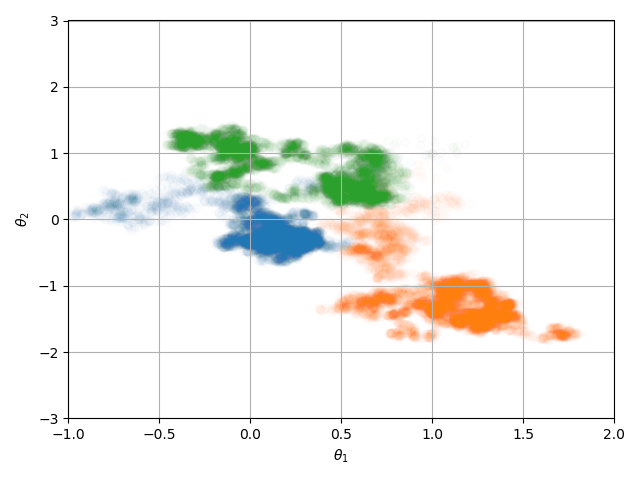
\includegraphics[width=0.49\linewidth]{poster-figures/gaussian_no_exchange.png}
  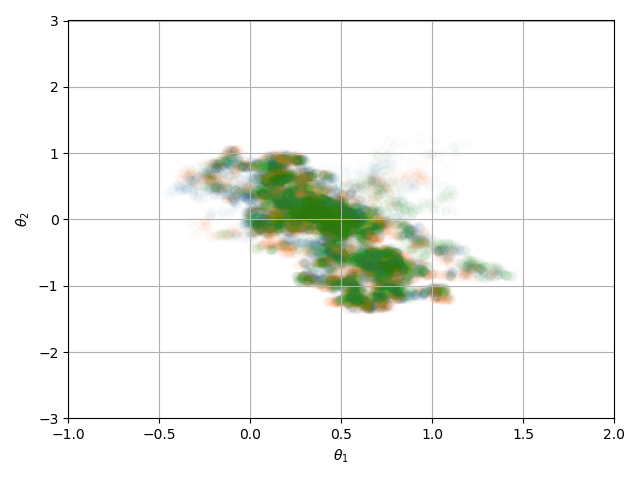
\includegraphics[width=0.49\linewidth]{poster-figures/gaussian_exchange.png}
  \caption{Samples drawn from local posteriors $P(\theta \mid X_s)$ (left, e.g.\ due to lack
    of chain exchange) may not well approximate the global posterior
    $P(\theta \mid \cup_s X_s)$ (right). Different colors corresponds to different chains.}
  \label{fig:samples}
\end{figure}

As we increase the number of workers $S$, we expect the rate at which samples are collected to increase.
Indeed, \cref{fig:speedup-partitioning} confirms that it takes less time to generate the same number
of samples when we have more workers. However, the scaling is not very good as
\cref{fig:speedup-partitioning} shows that the time to generate $800000$ samples is only cut down by
$\sim 1/3$ when three workers are added (perfect scaling would expect this to be a $2/3$ reduction).
We can attribute this poor scaling to communication overhead, which we will address in the following section.

\begin{figure}[htbp]
  \centering
  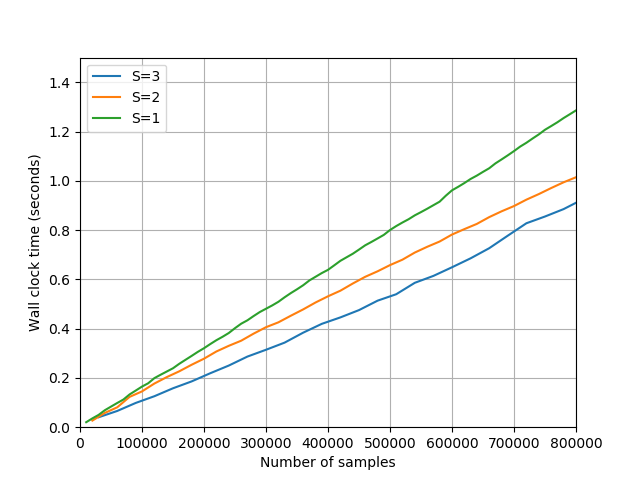
\includegraphics[width=0.5\linewidth]{poster-figures/speedup-parallel.png}
  \caption{Speedup in sampling due to parallelism.}
  \label{fig:speedup-partitioning}
\end{figure}

\section{Trajectory sampling}

As illustrated in \cref{fig:speedup-partitioning}, exchanging chains after each
iteration incurs significant communication overhead and impacts the algorithms
scaling behavior. To circumvent this, SGLD can be modified to perform
trajectory sampling. Instead of drawing a single sample, a trajectory of length
$\tau$ is sampled on each worker prior to exhanging chains. This can reduce the
amount of inter-worker communication by a factor of $1/\tau$,
but it must be used with care as too little chain exchange results in biased samples
(setting $\tau$ equal to the number of samples is equivalent to never exchanging chains).

\begin{figure}[htbp]
  \centering
  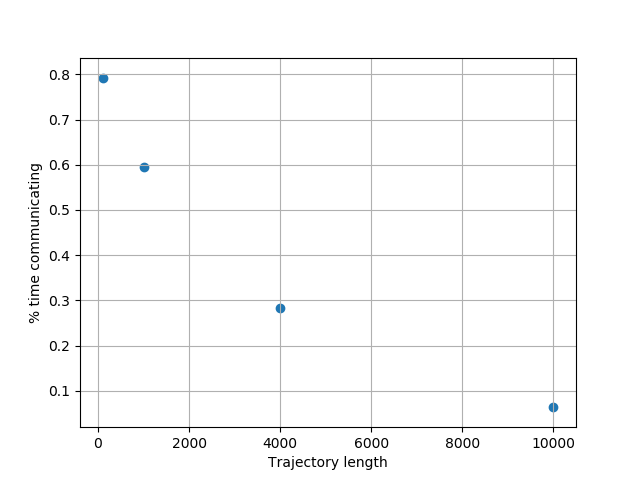
\includegraphics[width=0.5\linewidth]{poster-figures/traj_length_slowdown.png}
  \caption{Increasing trajectory length reduces how often communication happens, resulting in less
    communication overhead.}
  \label{fig:less-comm}
\end{figure}

\Cref{fig:less-comm} shows the fraction of time spent communication during an execution of the
algorithm. As expected, we see that longer trajectory lengths reduces this quantity and leads to
a greater proportion of time spent generating samples.

Although we do not explore it in this work, one interesting direction for
future work would be to explore the tradeoff between mixing rate and trajectory
length in more detail. For example, one could try to optimize $\tau$ by
choosing it such that it generates the largest effective sample size in a fixed
amount of time.

\section{Trajectory length load balancing}

Workers may not all finish sampling trajectories at the same times.
For example, workers may have different hardware and data partitioning may be imbalanced.
As a result, faster workers must block on slower workers on every chain exchange, leading to
low utilization (see \cref{fig:ahn-lb}).

\begin{figure}[htbp]
  \centering
  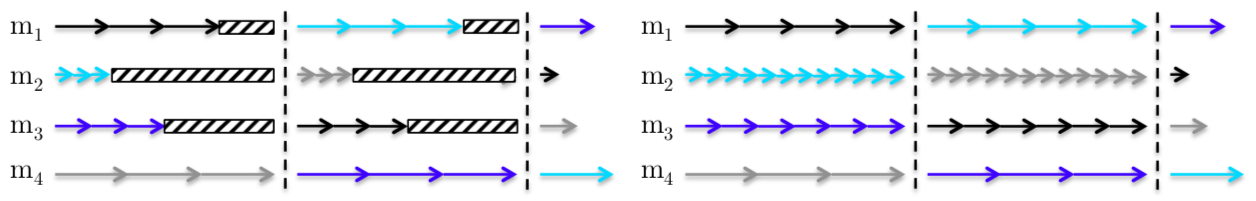
\includegraphics[width=1.0\linewidth]{poster-figures/ahn-lb.png}
  \caption{Figure from \cite{ahn2014distributed} illustrating trajectory length load balancing.
    The fast worker $m_2$ must sit idle waiting for the slow worker $m_4$ without load balancing (left),
    whereas after (right) it utilizes this time to generate a longer tarjectory.}
  \label{fig:ahn-lb}
\end{figure}

To improve utilization, we can modify the global trajectory length $\tau$ into
a worker-specific trajectory lengths $(\tau_s)_{s \in S}$ and use $\tau_s$ to
balance work. Faster workers can be assigned a larger $\tau_s$, allowing them
to continue generating samples while waiting. We set these worker-specific
trajectory lengths following \citet{ahn2014distributed} by reporting the time spent
within the trajectory sampling loop to the master and adjusting $\tau_s$ in an
inversely proportional manner. The results of this modification are shown in
\cref{fig:load-balancing}, where we simulated imbalanced data partitioning by
assigning 95\% of the data to worker 1. The reduction in latencies after the first
iteration (where initial timing results are gathered) confirm that trajectory load
balancing results in improved utilization.

\begin{figure}[htbp]
  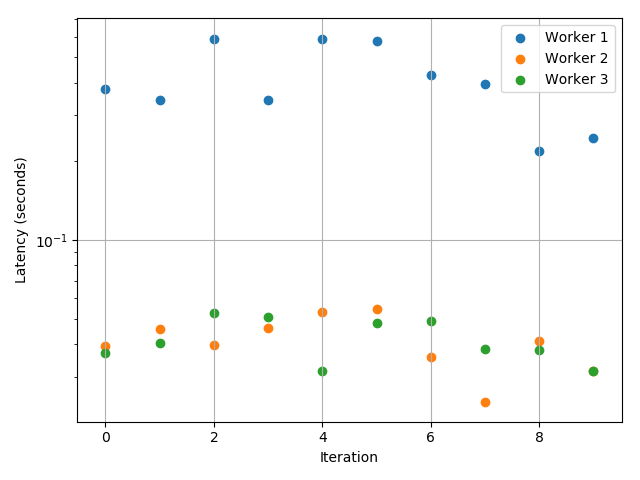
\includegraphics[width=0.49\linewidth]{poster-figures/load-balancing-none.png}
  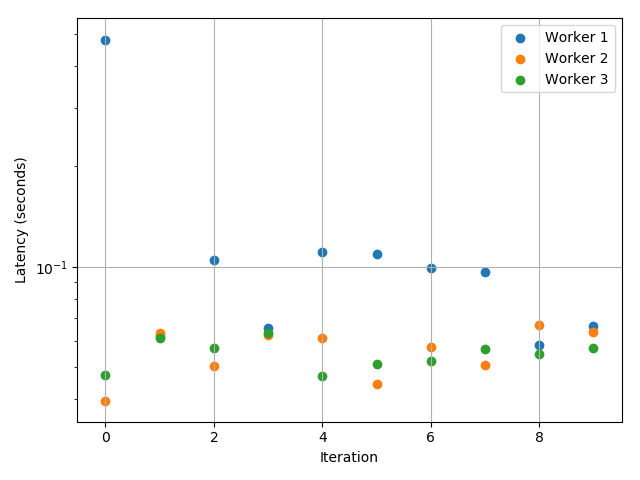
\includegraphics[width=0.49\linewidth]{poster-figures/load-balancing.png}
  \caption{Before (top) and after (bottom) trajectory length load balancing. Experiments used
    the GMM with an imbalanced data partitioning which assigned 95\% to worker 1. The lower variance
    in latency after the first iteration (where initial timing results are gathered)
    confirm that trajectory length load balancing results in improved
    utilization.}
  \label{fig:load-balancing}
\end{figure}

\section{Latent Dirichlet Allocation with Riemannian Langevin Dynamics}

So far, we have only explored a toy GMM. One real world application of posterior
sampling is inference in LDA \citep{blei2003latent}, a probabilistic topic model
used to discover structure in documents. As ``topics'' in LDA represent
discrete distributions over words, they are constrained to lie on the probability simplex.
Accordingly, we leverage stochastic gradient Riemannian Langevin dynamics \citep{patterson2013stochastic}
to sample the probability simplex and adapt it to run in a distributed MPI environment
over partitioned data. The result of training a LDA model using our implementation is shown in
\cref{fig:perplexity-sgrld}, where we see that the parameters sampled are decreasing in perplexity.
This indicates that the sampler is being drawn towards a posterior mode, and suggests that the implementation
is behaving as expected.

\begin{figure}[htbp]
  \centering
  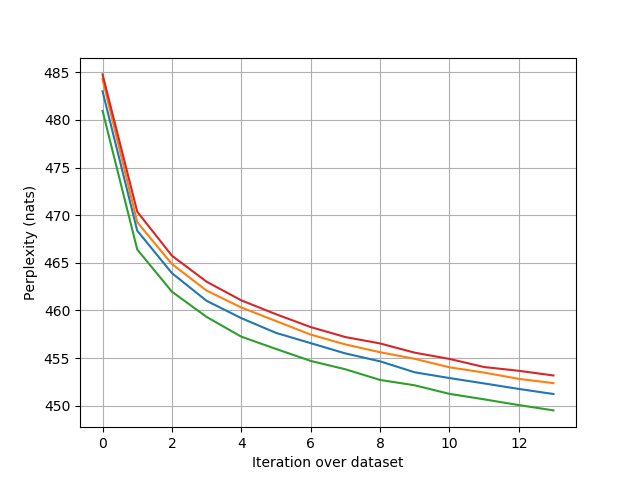
\includegraphics[width=0.5\linewidth]{poster-figures/perplexity-lda.png}
  \caption{Distributed SGRLD training on NIPS corpus ($1740$ documents,
    $19889$ unique words) of a 10 topic LDA model. Each color corresponds to a different chain.}
  \label{fig:perplexity-sgrld}
\end{figure}

\section{Conclusion}

We provide an implementation of D-SGLD on top of MPI and investigate the performance
characteristics of various optimizations. Our results demonstrate that D-SGLD enjoys
significant speedups due to parallelism, can sample posteriors even when data is partitioned
disjointedly across workers, and can be controlled using trajectory lengths to trade off
between communication versus mixing time as well as load balance workers.

\bibliographystyle{plainnat}
\bibliography{final-report}

\end{document}
